\documentclass[tikz,border=5pt]{standalone}
\usepackage{tikz}
\usetikzlibrary{arrows.meta,positioning}

\begin{document}
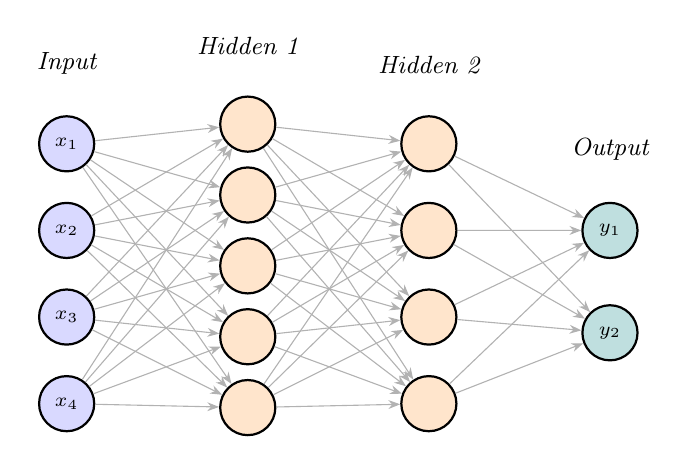
\begin{tikzpicture}[
    neuron/.style={circle, draw, minimum size=0.7cm, thick},
    input/.style={neuron, fill=blue!15},
    hidden/.style={neuron, fill=orange!20},
    output/.style={neuron, fill=teal!25},
    arrow/.style={-{Stealth[length=1.5mm]}, gray!60},
    label/.style={font=\small\itshape}
]

% Input layer
\foreach \i in {1,2,3,4} {
    \node[input] (i\i) at (0, -\i*1.1+2.2) {\scriptsize $x_{\i}$};
}

% Hidden layer 1
\foreach \i in {1,2,3,4,5} {
    \node[hidden] (h1\i) at (2.3, -\i*0.9+2.25) {};
}

% Hidden layer 2
\foreach \i in {1,2,3,4} {
    \node[hidden] (h2\i) at (4.6, -\i*1.1+2.2) {};
}

% Output layer
\foreach \i in {1,2} {
    \node[output] (o\i) at (6.9, -\i*1.3+1.3) {\scriptsize $y_{\i}$};
}

% Connections: input to hidden 1
\foreach \i in {1,2,3,4} {
    \foreach \j in {1,2,3,4,5} {
        \draw[arrow] (i\i) -- (h1\j);
    }
}

% Connections: hidden 1 to hidden 2
\foreach \i in {1,2,3,4,5} {
    \foreach \j in {1,2,3,4} {
        \draw[arrow] (h1\i) -- (h2\j);
    }
}

% Connections: hidden 2 to output
\foreach \i in {1,2,3,4} {
    \foreach \j in {1,2} {
        \draw[arrow] (h2\i) -- (o\j);
    }
}

% Layer labels
\node[label, above=0.4cm of i1] {Input};
\node[label, above=0.4cm of h11] {Hidden 1};
\node[label, above=0.4cm of h21] {Hidden 2};
\node[label, above=0.4cm of o1] {Output};

\end{tikzpicture}
\end{document}
